\documentclass{article}
\usepackage{enumerate}
\usepackage{fullpage}
\usepackage[fleqn]{amsmath}
\usepackage{amssymb}
\usepackage{graphicx}
\usepackage{hyperref}
\usepackage[english]{babel}
\usepackage{graphicx}

\setlength{\parindent}{0pt} 

\newcommand{\myspace}{0.4cm}
\pagestyle{empty}
\usepackage{array}
\newcolumntype{C}[1]{>{\centering\let\newline\\\arraybackslash\hspace{0pt}}m{#1}}
\newcolumntype{L}[1]{>{\raggedright\let\newline\\\arraybackslash\hspace{0pt}}m{#1}}
\newcolumntype{R}[1]{>{\raggedleft\let\newline\\\arraybackslash\hspace{0pt}}m{#1}}
\DeclareMathOperator\erf{erf}

\usepackage[framemethod=TikZ]{mdframed}
\mdfdefinestyle{MyFrame}{%
    innertopmargin=\baselineskip,
    innerbottommargin=\baselineskip,
    innerrightmargin=20pt,
    innerleftmargin=20pt,
    backgroundcolor=gray!10!white}

\def\name{Drake Bridgewater}

%% The following metadata will show up in the PDF properties
\hypersetup{
  colorlinks = true,
  urlcolor = black,
  pdfauthor = {\name},
  pdfkeywords = {mth351 ``Numerical Analysis''},
  pdftitle = {MTH 351: Homework 4},
  pdfsubject = {MTH 351: Homework 4},
  pdfpagemode = UseNone
}

\begin{document}
\hfill \name

\begin{center}

\large
\begin{tabular}{L{0.3\linewidth} C{0.3\linewidth} R{0.3\linewidth}}
\hline
Assignment 4    &MTH 351 -- Section 010        &\today \\
\hline
\end{tabular}
\vspace{-0.2cm}
\end{center}
\begin{enumerate}
%%%QUESTION 1
\item 
\begin{mdframed}[style=MyFrame]
\begin{enumerate}
\item Exponential Fit
If you separate the function $log(y) = Log(a) +b x$ into matrix from where x and y are actually many different points on a scatter plot then we get something like this. With this we can solve it using matrix math.\\
\begin{tabular}{p{1.5cm} p{1.3cm} p{1.3cm}}
\begin{equation*}
\begin{bmatrix}
1 & x\\
\vdots & \vdots \\
1 & x_n
\end{bmatrix}
\end{equation*}
&
\begin{equation*}
\begin{bmatrix}
log(y)\\
b
\end{bmatrix}
\end{equation*}
&
\begin{equation*}
=\begin{bmatrix}
log(y)\\
\vdots \\
log(y)
\end{bmatrix}
\end{equation*}
\vspace{-.1cm}
\end{tabular}
\begin{verbatim}
A = [ones(size(x)) x] ;
coeffs = A\log(y);
plot(x, exp(coeffs(1)+(coeffs(2) * x)), 'g-', 'Linewidth', 2)
\end{verbatim}
\item Power Fit
If you separate the function $log(y) = Log(a) + b log(x)$ into matrix from where x and y are actually many different points on a scatter plot then we get something like this. With this we can solve it using matrix math.\\
\begin{tabular}{p{3cm} p{1.5cm} p{1.5cm}}
\begin{equation*}
\begin{bmatrix}
1 & log(x)\\
\vdots & \vdots \\
1 & log(x_n)
\end{bmatrix}
\end{equation*}
&
\begin{equation*}
\begin{bmatrix}
log(a)\\
b
\end{bmatrix}
\end{equation*}
&

\begin{equation*}
=\begin{bmatrix}
log(y)\\
\vdots \\
log(y)
\end{bmatrix}
\end{equation*}

\end{tabular}
\begin{verbatim}
A= [ones(size(x)) log(x)];
coeffs = A\log(y);
plot(x, exp(coeffs(1) + coeffs(2) * log(x)), 'b-', 'Linewidth', 2)
\end{verbatim}

\begin{center}
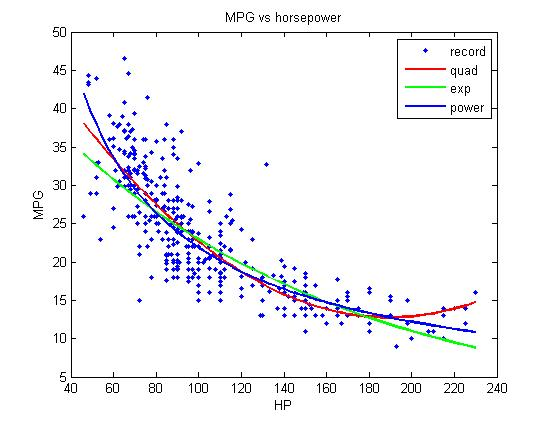
\includegraphics[width=0.7\textwidth]{a4q11.jpg}\\
\end{center}
  Just by a visual stand point it is difficult to see which best fit actually looks and works the best, but a closer look and the quadratic function starts to increase towards the end and from my expertise in fuel economy it does not work that way. Therefore I would discredit the quadratic function engines with large horse power. The exponential equation has the smallest slope and estimates nearly all values rather low. Whereas the power function starts the highest and and stays in the middle of the other two functions.
\end{enumerate}
\end{mdframed}

\item 
\begin{mdframed}[style=MyFrame]
\begin{enumerate}
\item For what function, $f(x)$ do you need to find a root?  $y=x^3-20$\\
\begin{tabular}{p{6cm} p{6cm}}

\item How many iterations of bisection must you have to produce a result with an error less then $10^{-6}$? you must have 20 because &
\begin{equation}
\frac{ln(\frac{b-a}{\epsilon}}{ln(2)} < n
\end{equation}
\end{tabular}\\ \vspace*{-0.3cm}
\begin{tabular}{p{6cm} p{6cm}}

How many iterations of bisection must you have to produce a result with an error less then $10^{-6}$? you must have 20 because &
\begin{equation}
\frac{ln(\frac{b-a}{\epsilon}}{ln(2)} < n
\end{equation}
\end{tabular}
\\
\begin{tabular}{p{6cm} p{6cm}}
This equation (1) produces 19.93 with a=2, b=3, and $\epsilon=10^{-6}$ &
\begin{equation} 
\frac{ln(\frac{3-2}{10^{-6}}}{ln(2)} = 19.93
\end{equation}
\end{tabular}

Since we are looking for greater precision we are going to round up yielding 20 iterations of the bisection
\newpage\item Changing the function, $f = @(x) x^3 - 20$ that bisect.m operates on produce an iteration table of 
\begin{verbatim}
>> bisect(2,3,10^-6,20)
   n          a                  b                  c                   f(c)
-------    -------------    -------------    -------------    -------------
  1    2.00000000e+00    3.00000000e+00    2.50000000e+00    -4.37500000e+00
  2    2.50000000e+00    3.00000000e+00    2.75000000e+00    7.96875000e-01
  3    2.50000000e+00    2.75000000e+00    2.62500000e+00    -1.91210938e+00
  4    2.62500000e+00    2.75000000e+00    2.68750000e+00    -5.89111328e-01
  5    2.68750000e+00    2.75000000e+00    2.71875000e+00    9.59167480e-02
  6    2.68750000e+00    2.71875000e+00    2.70312500e+00    -2.48577118e-01
  7    2.70312500e+00    2.71875000e+00    2.71093750e+00    -7.68265724e-02
  8    2.71093750e+00    2.71875000e+00    2.71484375e+00    9.42081213e-03
  9    2.71093750e+00    2.71484375e+00    2.71289063e+00    -3.37339267e-02
 10    2.71289063e+00    2.71484375e+00    2.71386719e+00    -1.21643217e-02
 11    2.71386719e+00    2.71484375e+00    2.71435547e+00    -1.37369626e-03
 12    2.71435547e+00    2.71484375e+00    2.71459961e+00    4.02307253e-03
 13    2.71435547e+00    2.71459961e+00    2.71447754e+00    1.32456679e-03
 14    2.71435547e+00    2.71447754e+00    2.71441650e+00    -2.45950703e-05
 15    2.71441650e+00    2.71447754e+00    2.71444702e+00    6.49978275e-04
 16    2.71441650e+00    2.71444702e+00    2.71443176e+00    3.12689706e-04
 17    2.71441650e+00    2.71443176e+00    2.71442413e+00    1.44046844e-04
 18    2.71441650e+00    2.71442413e+00    2.71442032e+00    5.97257684e-05
 19    2.71441650e+00    2.71442032e+00    2.71441841e+00    1.75653194e-05
 20    2.71441650e+00    2.71441841e+00    2.71441746e+00    -3.51488282e-06

ans =   2.714417457580566
\end{verbatim}

\item Run same equation in the newtons.m script and compare the results, is the convergence quadratic? To solve this problem you take the derivative twice. \\
\begin{tabular}{p{6cm} p{6cm}}
\begin{equation}
\frac{d}{dx}(x^3 - 20) = 3x^2
\end{equation} 
&
\begin{equation}
\frac{d}{dx} (3x^2) = 6x
\end{equation}
\end{tabular}\\
From trying different values that are close to the actual root and some from further I have came to the conclusion that this function cannot be solved in a reasonable number of iterations with the Netwon Method. 
\end{enumerate}
\end{mdframed}

\newpage\item
\begin{mdframed}[style=MyFrame]
\begin{enumerate}
\item Explain how to use Newton's method to find the point (x, y) on the graph of the function $y=x^2$ that is closest to the point (1,0)? To find the closes point on the equation of $y=x^2$ and the distance formula. The idea is that we want to find the minimum distance to find the minimum distance we can use the distance formula from the point (1,0) and the function $y=x^2$. 

\begin{equation}
D(x) = \sqrt{(x-a)^2-(y(x)-b)^2}
\end{equation}
Plugging in our values for the point (1,0) and the function $y=x^2$.
\begin{equation}
D(x) = \sqrt{(x-1)^2-(x^2-0)^2} = \sqrt{(x-1)^2-x^4}
\end{equation}
In order to use Newton's method $x_{x+n}=x_n-\frac{f(x_n)}{f'(x_n)}$ we must find the first and the second derivative. 
\begin{equation}
    D'(x)  = \frac{2 x^3+x-1}{\sqrt{x^4+x^2-2  x+1}}
\end{equation}

\begin{equation}
    D''(x) = \frac{(x^2) (2x^4+3 x^2-8 x+6)}{(x^4+x^2-2 x+1)^{3/2}}
\end{equation}
Once the two derivative have been found calculate the x value is fairly straight forward with the newtons.m script.
\begin{verbatim}
>> newtons(.5,10^-6,20)
f =  @(x)(2*x^3+x-1)/sqrt(x^4+x^2-2*x+1)
fp = @(x)((x^2)*(2*(x^4)+3*(x^2)-8*x+6))/((x^4)+(x^2)-2*x+1)^(3/2)

 n          x                  f(x)          quad. ratio       lin. ratio
---   -------------     -------------      -------------      -------------
 0    5.00000000e-01    -4.47213595e-01
 1    6.08695652e-01    1.10880405e-01
 2    5.90085840e-01    1.90232858e-03    -1.57513450e+00    -1.71210271e-01
 3    5.89754638e-01    7.19739262e-07    -9.56333713e-01     1.77971907e-02
 4    5.89754512e-01    1.03210995e-13    -1.14320785e+00     3.78633153e-04
ans =   0.589754512301476
\end{verbatim}
\item Use newtons.m to find the value of (x,y)? To find the the value of x and y all you have to do is plug in the value we got for the answer which coorlates to the x value into the equation $y=x^2$. Therefore the result is $y=0.5897545^2=0.34781028$

\end{enumerate}
\end{mdframed}

\end{enumerate}

\end{document}

